\documentclass{article}%
\usepackage{amsmath}
\usepackage{graphicx}
\usepackage{amsfonts}
\usepackage{amssymb}%
\setcounter{MaxMatrixCols}{30}

\providecommand{\U}[1]{\protect\rule{.1in}{.1in}}
%EndMSIPreambleData
\providecommand{\U}[1]{\protect\rule{.1in}{.1in}}
\providecommand{\U}[1]{\protect\rule{.1in}{.1in}}
\newtheorem{theorem}{Theorem}
\newtheorem{acknowledgement}[theorem]{Acknowledgement}
\newtheorem{algorithm}[theorem]{Algorithm}
\newtheorem{axiom}[theorem]{Axiom}
\newtheorem{case}[theorem]{Case}
\newtheorem{claim}[theorem]{Claim}
\newtheorem{conclusion}[theorem]{Conclusion}
\newtheorem{condition}[theorem]{Condition}
\newtheorem{conjecture}[theorem]{Conjecture}
\newtheorem{corollary}[theorem]{Corollary}
\newtheorem{criterion}[theorem]{Criterion}
\newtheorem{definition}[theorem]{Definition}
\newtheorem{example}[theorem]{Example}
\newtheorem{exercise}[theorem]{Exercise}
\newtheorem{lemma}[theorem]{Lemma}
\newtheorem{notation}[theorem]{Notation}
\newtheorem{problem}[theorem]{Problem}
\newtheorem{proposition}[theorem]{Proposition}
\newtheorem{remark}[theorem]{Remark}
\newtheorem{solution}[theorem]{Solution}
\newtheorem{summary}[theorem]{Summary}
\newenvironment{proof}[1][Proof]{\textbf{#1.} }{\ \rule{0.5em}{0.5em}}
\begin{document}
\begin{center}
\textbf{Math 21-269, Vector Analysis I, Spring 2024}
\textbf{Assignment 1}
\end{center}
\textbf{The due date for this assignment is Friday, January 26.}
\begin{enumerate}
\item Let $G\subseteq\mathbb{R}$ be an additive group. Prove that the
following two conditions are equivalent:
\begin{enumerate}
\item for every $0<x<y$ there exists $g\in G$ such that $x<g<y$,
\item $\inf\{g\in G:\,g>0\}=0$.
\end{enumerate}
\item
\[
f\left( x\right) =\arcsin\frac{1-x^{2}}{1+x^{2}},
\]
\begin{enumerate}
\item find the domain $D$ of $f$,
\item find its derivative and the sets in which $f$ is increasing,
\item sketch the graph of $f$,
\item find the supremum and the infimum of the set%
\[
E=\left\{ y\in\mathbb{R}:\,y=\arcsin\frac{1-x^{2}}{1+x^{2}},\,x\in D\right\}
.
\]
\end{enumerate}
\end{enumerate}
\begin{center}
\textbf{JUSTIFY\ ALL\ YOUR\ ANSWERS}

\textbf{Solutions}
\begin{enumerate}
    \item 
    \begin{proof}We start by showing $(a) \implies (b)$. We need to prove that for all $\epsilon >0$, there exists $g \in G$ such that $0 < g < \epsilon$. This is saying that there is no positive $g < \epsilon$ that is a lower bound, and therefore the infimum is 0. Fix $x = \dfrac{\epsilon}{2}$ and $y = \epsilon$ for $\epsilon > 0$ (which means $\dfrac{\epsilon}{2} >0$). By condition (a), there exists $g \in G$ such that $\dfrac{\epsilon}{2} < g < \epsilon$. This yields that $ 0 < g < \epsilon$ as desired. Thus, we have shown that (a) $\implies$ (b).
    $$$$
    Now, we show that (b) $\implies$ (a). We need to prove that for all $0 < x< y$, there exists $g \in G$ such that $x < g < y$. Given any $0 < x < y$, choose $\epsilon$ such that $0 < \epsilon < y-x$. We know that there is an $\epsilon \in \{g \in G : g > 0\}$ that suffices this inequality because if there weren't, that would mean $y-x$ would be a lower bound of $\{g \in G : g > 0\}$, which contradicts the fact that the infimum is 0. 

    Consider the element $\epsilon \left\lfloor \dfrac{x}{e} \right\rfloor + \epsilon$, which we know is in $G$ because it is an additive group (multiplication is repeated addition). Then, we have:
    \begin{align*}
        x < \epsilon \left\lfloor \dfrac{x}{e} \right\rfloor  + \epsilon \leq x + \epsilon < x + (y-x) = y
    \end{align*}
    Thus, we have shown that (b) $\implies$ (a).
    $$$$
    Therefore, we have shown that (a) and (b) are equivalent.
    \end{proof}
    \item \begin{enumerate}
        \item The argument of arcsin needs to be in $[-1, 1]$. So, we are limited to points where $\dfrac{1-x^2}{1+x^2} \in [-1, 1]$. I claim that this is true for all $x \in \mathbb{R}$. 
        \begin{proof}
        If $\dfrac{1-x^2}{1+x^2} < -1$, we have the following:
        \begin{align*}
            \dfrac{1-x^2}{1+x^2} &< -1 \\
            1 - x^2 &< -1 - x^2 \\
            1 &< -1
        \end{align*} The above is a contradiction.
        If we have $\dfrac{1-x^2}{1+x^2} > 1$, we have the following:
        \begin{align*}
            \dfrac{1-x^2}{1+x^2} &> 1 \\
            1 - x^2 &> 1 + x^2 \\
            1 &> 2
        \end{align*} The above is another contradiction. 

        Thus, we have that $\dfrac{1-x^2}{1+x^2} \in [-1, 1]$ for all $x \in \mathbb{R}$. Thus, the domain of $f$ is $\mathbb{R}$.
    \end{proof}
        \item Finding the derivative:
        \begin{align*}
            f(x) &= \arcsin \frac{1-x^2}{1+x^2} \\
            f'(x) &= \dfrac{d}{dx} \arcsin \frac{1-x^2}{1+x^2} \\
            &= \dfrac{1}{\sqrt{1 - \left(\frac{1-x^2}{1+x^2}\right)^2}} \cdot \dfrac{d}{dx} \left(\frac{1-x^2}{1+x^2}\right) \\
            &= \dfrac{\dfrac{\dfrac{d}{dx}(1-x^2)(1+x^2) - (1-x^2)\cdot \dfrac{d}{dx}(1+x^2)}{(x^2+1)^2}}{\sqrt{1 - \left(\frac{1-x^2}{1+x^2}\right)^2}} \\
            &= \dfrac{(-2x)(1+x^2) - (1-x^2)(2x)}{(x^2+1)^2 \sqrt{1 - \left(\frac{1-x^2}{1+x^2}\right)^2}} \\
            &= \boxed{\dfrac{-4x}{(x^2+1)^2 \sqrt{1 - \left(\frac{1-x^2}{1+x^2}\right)^2}}} \\
        \end{align*}
        We can see that $f'(x) < 0$ when $ x < 0$. This is because the denominator is always positive (a squared value multiplied by a square rooted value, both of which are for sure positive). Though this is not the case when $x =0$, which makes the square root value $0$ and therefore $f$ is indifferentiable at $x=0$. However, we still only need to analyze the sign of $-4x$, which is positive when $x$ is negative and vice versa. Therefore, $f$ is increasing on $(-\infty, 0)$.
        \item Here are some key facts we need to realize before sketching:
        \begin{enumerate}
            \item $f$ is defined for all $x \in \mathbb{R}$.
            \item $f$ is increasing on $(-\infty, 0)$ and vice versa.
            \item $f$ is limited by the range of arcsin, which is $\left[-\dfrac{\pi}{2}, \dfrac{\pi}{2}\right]$. Since the argument of arcsin has an asymptote at $y = -1$, we can say that $f$ has an asymptote at $y = -\dfrac{\pi}{2}$.
        \end{enumerate}
        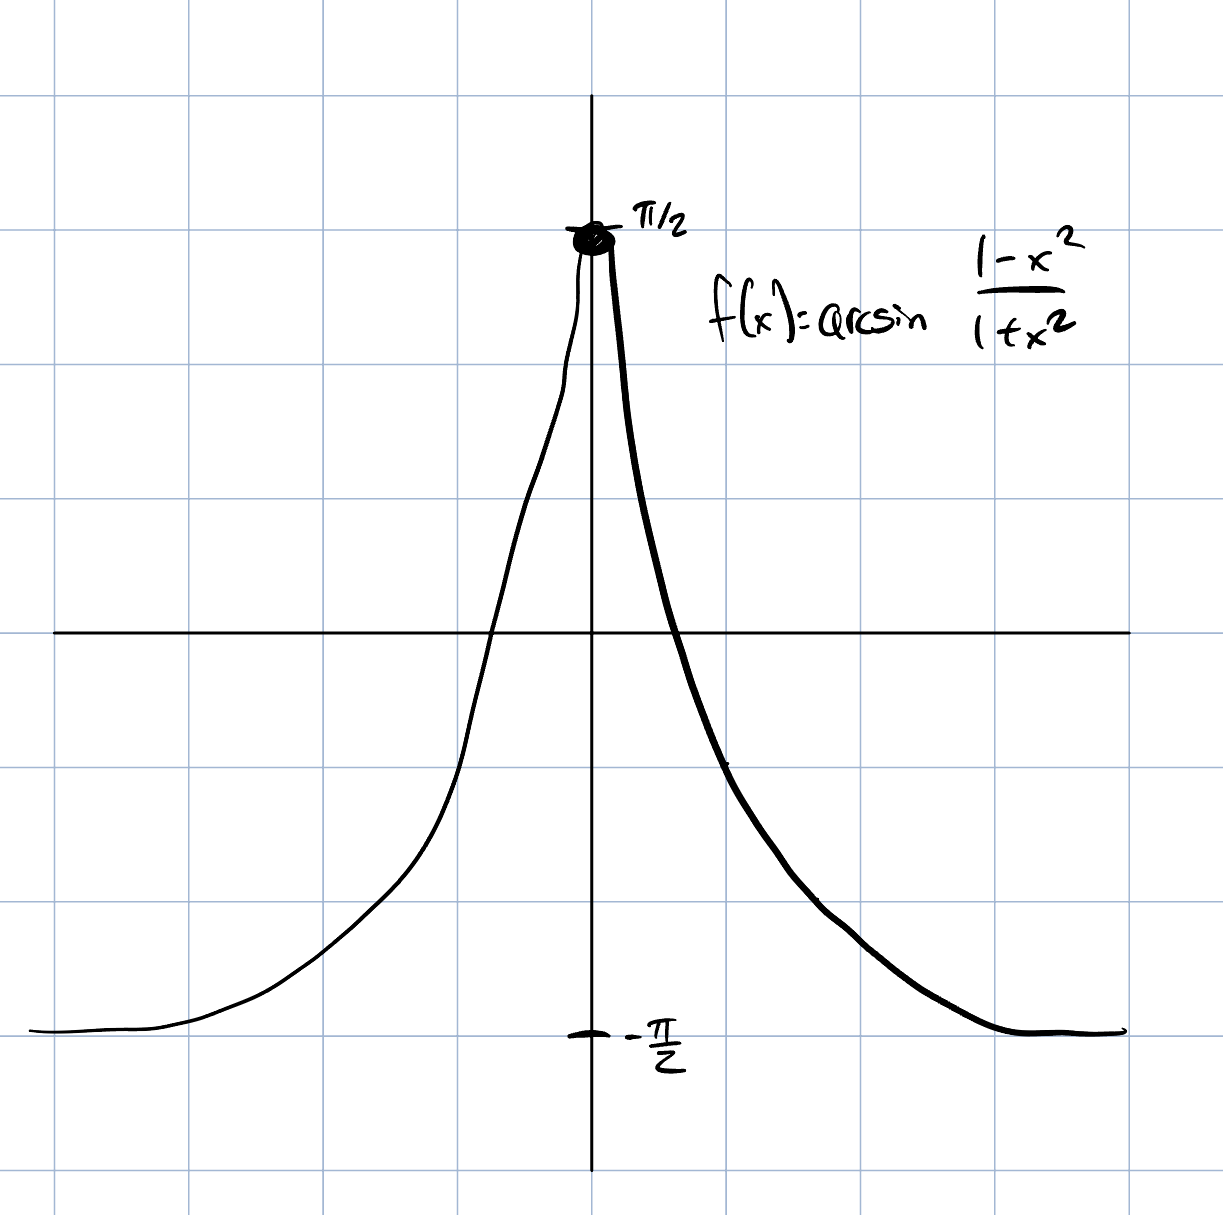
\includegraphics[scale=0.3]{hw1_2c.png}
        \item I claim that the supremum is $\dfrac{\pi}{2}$ and the infimum is $-\dfrac{\pi}{2}$.
        
        \textbf{Supremum:} $\arcsin(z)$ as a function is bounded above by $\dfrac{\pi}{2}$, which occurs when $z = 1$. We can see that $z = \dfrac{1-x^2}{1+x^2}$, which equals 1 when $x = 0$. Thus, the supremum is $\dfrac{\pi}{2}$.

        \textbf{Infimum:} $\arcsin(z)$ as a function is bounded below by $-\dfrac{\pi}{2}$, which occurs when $z = -1$. Since the horizontal asymptote of $z = \dfrac{1-x^2}{1+x^2}$ is $y = -1$, we can say that $z$ approaches, but never reaches $-1$. This means that for $f$, we approach, but never cross $-\dfrac{\pi}{2}$. Thus, the infimum is $-\dfrac{\pi}{2}$.

        If we want to be more rigorous, let $y = -\dfrac{\pi}{2} + \epsilon$ for $\pi \geq \epsilon \geq 0$.
        \begin{align*}
            -\dfrac{\pi}{2} + \epsilon &= \arcsin \frac{1-x^2}{1+x^2} \\
            \sin\left(-\dfrac{\pi}{2} + \epsilon\right) &= \frac{1-x^2}{1+x^2} \\
            -\cos(\epsilon) &= \frac{1-x^2}{1+x^2} \\
            -\cos(\epsilon)(1+x^2) &= 1-x^2 \\
            -\cos(\epsilon) - x^2\cos(\epsilon) &= 1-x^2 \\
            x^2\cos(\epsilon) - x^2 &= 1 + \cos(\epsilon) \\
            x^2(\cos(\epsilon) - 1) &= 1 + \cos(\epsilon) \\
            x^2 &= \frac{1 + \cos(\epsilon)}{\cos(\epsilon) - 1} \\
            x &= \pm \sqrt{\frac{1 + \cos(\epsilon)}{\cos(\epsilon) - 1}}
        \end{align*}
        The only time this value will be undefined is when the denominator of the square root is equal to 0. This happens when $\cos(\epsilon) = 1 \Rightarrow \epsilon = 0$. Thus, we have that $x = \pm \sqrt{\dfrac{1 + \cos(\epsilon)}{\cos(\epsilon) - 1}}$ is defined for all $\pi \geq \epsilon > 0$. Thus, we have that $-\dfrac{\pi}{2} + \epsilon$ is in the range of $f$ for all $\pi \geq \epsilon > 0$. Thus, the infimum is $-\dfrac{\pi}{2}$.
    \end{enumerate}
\end{enumerate}
\end{center}
\end{document}